\documentclass[conference]{IEEEtran}

\usepackage{url}
\usepackage{amsmath}
\usepackage[pdftex]{graphicx}
\usepackage{balance}
\usepackage{caption}
\usepackage{subcaption}
\usepackage{paralist}

\newcommand{\comment}[1]{{\textcolor{blue}{#1}}}


\usepackage{color,soul}

\newcommand{\todo}[1]{\hl{TODO:~#1}}
\renewcommand*\ttdefault{txtt} % the more modern typewriter

%%%%%%%%%%%%%%%%%%%%%%%%%%%%%%%%%%%%%%%%%%%
\begin{document}


\title{SLOC: Service Level Objectives for Next Generation Cloud Computing \\
%SUBTITLE
\Large{Vision, Research Challenges and Approach Overview}
}

\author{
	\IEEEauthorblockN{Stefan Nastic, Andrea Morichetti, \\ Thomas Pusztai, Schahram Dustdar}
	\IEEEauthorblockA{Distributed Systems Group, \\TU Wien, Vienna, Austria} 
									
\and	
	\IEEEauthorblockN{\todo{Futurewei Team}}
	\IEEEauthorblockA{Futurewei Technologies, Inc., \\ Santa Clara CA USA}
}

% \IEEEoverridecommandlockouts

\maketitle
\begin{abstract}
In this paper we outline research challenges, approaches, vision and road map for the SLOC project ....

\todo{NOTE: IC papers have a limit of 5000 words or ca. 5.5 pages IEEE style.}
\end{abstract}

\begin{IEEEkeywords}
Service Level Objectives, Cloud Computing, Elasticity, Data Analytics 
\end{IEEEkeywords}

% Include expernal sections
\section{Introduction}
%!TEX root = ../main.tex
\section{Background}
\label{sec:Background}

This paper builds on our previous research in the 
fields of elastic computing, SLAs and cloud engineering.
In the continuation, we outline the most important
aspects of our previous work underpinning this work.

\subsection{\em Elastic Computing.}
\todo{TUW: MELA, SYBL, multi dimensional elasticity}

\subsection{Cloud Engineering.}
\todo{FUW: arktos, etc}

%!TEX root = ../main.tex
\section{Research Challenges}
\label{sec:Challenges}

\begin{itemize}
	\item [\textbf{RC-1}] -- 
	Currently most of cloud platforms provide a very rudimentary
	support for specifying QoS and SLOs to end users. The vast majority 
	of models is based on the concepts of resource quotas, such as
	requests/limits in Kubernetes or templates/types in AWS. Unfortunately,
	correctly mapping desired workload's performance model to 
	resource quotas is a very challenging task in practice.
	
	\item [\textbf{RC-2}] -- 
	Vast majority of cloud platforms allow for specifying resource guarantees,
	but very few offer any support for additional elasticity dimensions,
	such as cost or quality. This significantly limits the end user (consumer)
	who might care more to optimize for the costs of executing a specific workload.
	Unfortunately, apart from some niche solutions (e.g., AWS Spot Instances)
	there is very limited support for multi-dimensional elasticity concerns 
	and optimization.
	
	\item [\textbf{RC-3}] -- 
	Latency-sensitive applications greatly benefit from NUMA aware 
	resource allocation. Other types of workloads such as CUP-bound, 
	ML-heavy workloads can benefit from CPU affinity such as GPU pinning.
	While there is usually a general support for node affinity, the 
	end user needs to	deal with too many low level details such
	as writing node selection expressions, which usually relay 
	on cluster specific features, hence making workloads hardly portable.
	Additionally, specifying such QoS requirements is very challenging task
	as it requires deep knowledge about both infrastructure setup specifics
	and cloud platform.
	
	\item [\textbf{RC-4}] -- 
	Observability is foundational element that needs to be considered 
	when building modern cloud-native and microservice applications.
	\todo{Finish}
	
	\item [\textbf{RC-5}] -- 
	%Cloud computing promises easy and quick consumption of infrastructure resources. 
	While there are numerous tools supporting infrastructure 
	provisioning and configuration management, support for run time elastic
	controlling remains fairly limited. It mainly bases on a notion 
	of autoscaling groups/sets of resources where a user specifies their cardinality.
	Most of the solutions only allow for service-level scaling policies 
	as opposed to full-stack scaling strategies. On the one hand, this 
	makes dealing with elasticity concerns cumbersome. On the other hand,
	synchronizing scaling actions across multiple services and 
	defining consistent and congruent scaling strategies becomes 
	very difficult. Finally, optimizing scaling actions 
	for specific elasticity and SLO dimensions, such as cost,	
	has only a rudimentary support.
	%eg AWS AutoScaling (but only a few templates with target scaling strategy...}
	Therefore, creating suitable elastic scaling strategies to date remains
	a challenging task.
	
	%\todo{Finish. Policies must be specified pro service
	%(application deployment segment), synchronizing scaling actions 
	%of multiple services is hard (consistent and congruent scaling strategies), 
	%optimizing for specific SLO such as cost 
	%is little supported eg AWS AutoScaling (but only a few 
	%templates with target scaling strategy...}	
\end{itemize}
%!TEX root = ../main.tex
\section{SLOC Approach Overview}
\label{sec:Approach}

\subsection{Main Objectives} 
To address the aforementioned challenges and 
achieve our vision of SLO-native paradigm for the next generation cloud
platforms, our SLOC framework sets the following main objectives.
\todo{Map the challenges to objectives}

\begin{itemize}
	\item \todo{We want to enable the users to specify the SLOs in terms which are aligned with their business requirements. The customers are interested in their app performance (business requirements) and don't care 
	about resources per se. For example, the costs can be the main decision driving factor.} 
	\item \todo {We are intending to use elasticity mechanisms to support and enforce/guarantee SLOs}
	\item In order to achieve formally verifiable requirements of both the Cloud 
elasticity and the application (e.g., SLOs), our framework intends to develop 
{\em SLO-native elasticity models}. This will facilitate formal reasoning on and 
verification of multidimensional elasticity and SLOs, from the early stages 
of design. 
\item In order to enable the shift from low-level, resource-centered SLOs 
and elastic requirements specification to {\em intent-focused, 
multidimensional elasticity models and performance-centered SLOs}, 
our framework will provide novel 
coordination, control, and orchestration approaches that enable Cloud systems 
to adapt dynamically to varying load patterns in a dependable manner.
\end{itemize}

\subsection{Main Concepts and Architecture Overview}
The core idea behind SLOC framework is to enable SLO-native management of 
elastic Cloud resources. 
\todo{In a nutshell,} our {\em SLO-native approach} introduces a 
paradigm shift from general, business logic agnostic, low-level SLAs to  
{\em intent-based, SLO-first, performance-driven and orchestration-aware} 
elasticity models.

\begin{enumerate}
	\item Intent-based means that we are declaring what the execution environment
	of a workload should look like i.e., the infrastructure/resource desired state for 
	the given point in time considering the elasticity requirements, constraints and SLAs.
	\item SLO-first means that all the SLOs and QoS along multiple elasticity 
	dimensions are inherently aligned with application model and business 
	requirements/KPIs as opposed to external, business logic agnostic configurations.
	\item Performance driven
	\item Orchestration-aware implies that the application deployment bundles
	such as microservices or service mashes are aware of automated deployment, 
	scaling, scheduling and management.
\end{enumerate}
%
\begin{figure}[t]  
\centering
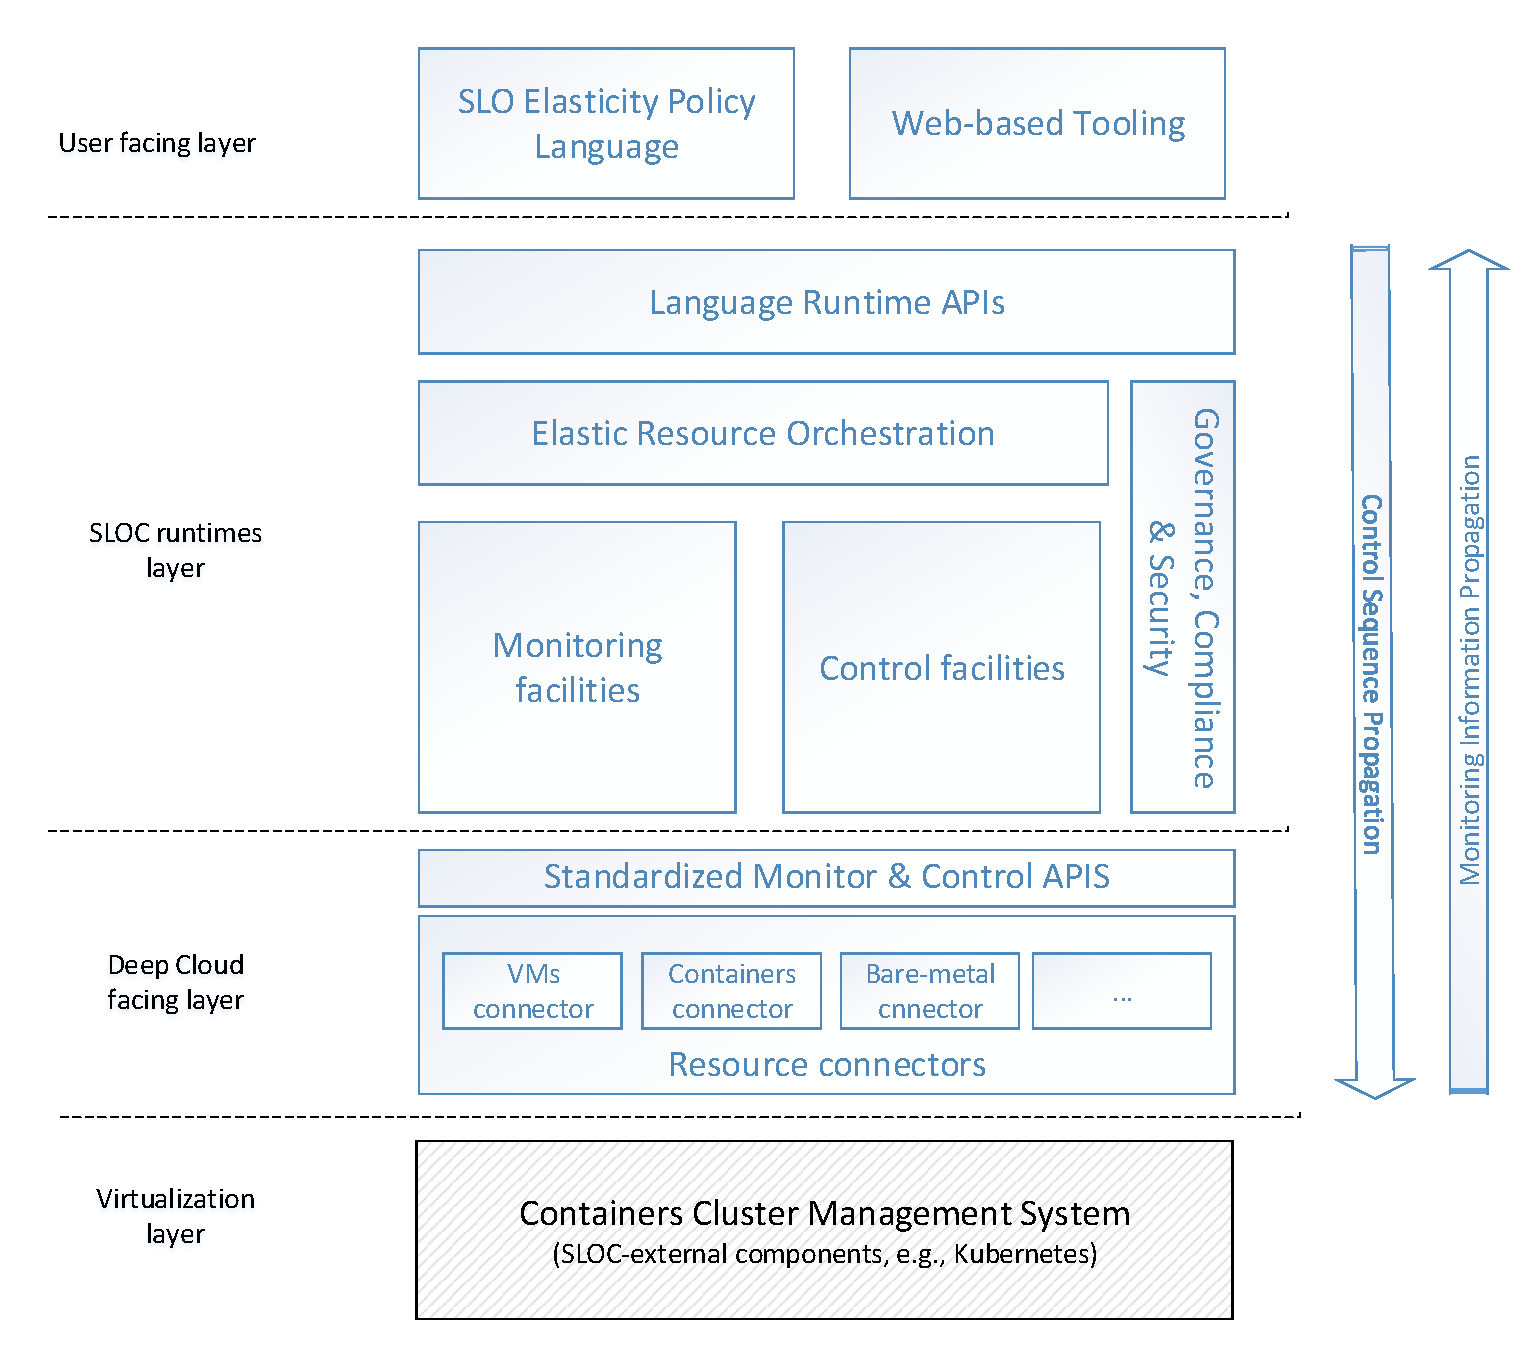
\includegraphics[width=0.8\columnwidth]{figures/sloc_architecture}
\caption{SLOC Architecture Overview.}
\label{fig:architecture}
\end{figure}% 
%
Subsequently, we outline the architecture of our SLOC framework
and give an overview of its main components.
Figure~\ref{fig:architecture} shows a high-level view of the 
framework architecture together with main control 
processes (top-down) and monitoring data delivery and analytics
process (bottom-up).
%
On a high-level we identify three main layers of SLOC framework:
\begin{inparaenum}[i)]
  \item User-facing layer,
  \item SLOC runtimes layer, and
  \item Deep Cloud facing layer.
\end{inparaenum}

The User-facing layer exposes main abstractions, mechanisms
and runtime services of the SLOC framework to the end users,
enabling them to define SLO elastic policies, visualize their
infrastructure and its current status, as determined by SLOC's
observability mechanisms. We discuss SLOC's SLO Elastic 
Policy Language in detail in Section~\ref{sec:mechanisms}.

The SLOC runtimes layer is the ``brains'' of our framework.
Generally, it is responsible for implementing main models, algorithms and
mechanisms, which are required to interpret user-defined SLOs,
translates such SLOs and QoS requirements in cloud-specific
resource \todo{configurations} and enforce such SLOs during runtime.
The most important components at this layer include:
\begin{inparaenum}[i)]
  \item Elastic Resource Orchestration,
  \item Observability facilities, 
  \item Control facilities, and
	\item Governance, Compliance \& Security Concerns.
\end{inparaenum}
%
The Elastic Resource Orchestration is responsible for interpreting and 
executing user-defined SLOs, elasticity requirements and 
configuration models.  
This layer acts as a ``gluing'' component bringing together SLO 
definitions, multi-dimensional elasticity models and framework's 
runtime mechanisms. For example, Elastic Resource 
Orchestration receives policy configuration directives, 
in terms of high-level objectives such as to optimize 
infrastructure for latency. It interprets these objectives 
and decides how to orchestrate the underlying resources, 
by invoking the underlying  runtime mechanisms as well as 
delegating specific decisions and/or responsibilities
to cluster management system controllers. 
%For example, it can utilize the Scheduling and 
%the Placement mechanisms to determine the most suitable 
%node for a service in order to reduce the network latency.
The details of Observability and Control facilities are
discussed in Section~\ref{sec:mechanisms}.

SLOC's third key layer is the Deep Cloud facing layer.
\todo{finish}


%!TEX root = ../main.tex
\section{Design Considerations for SLO-driven Elasticity Mechanisms}
\label{sec:mechanisms}

\subsection{SLO Elasticity Policy Language}
\todo{add}

\subsection{SLOC Observability}
\todo{add}
\todo{Which metrics are needed from user but also from providers perspective}

\subsection{SLOC Elasticity Controlling}
\todo{add}

\subsection{Implementation Considerations}
\todo{add}
Next we discuss preliminary solution
design and implementation considerations of our SLOC framework.
In general, the SLOC framework aims to build on and extend our previous
work and frameworks: Arktos, MELA and SYBL.
%
As Arktos evolved from the Kubernetes codebase, introducing several fundamental 
improvements, we intend to continue the development of SLOC framework
in the same direction, effectively aligning it both with Arktos and Kubernetes.

\todo{Outline the implementation on top of Arktos/Kubernetes}


\subsection{Governance and Compliance}
\todo{add}
%!TEX root = ../main.tex
\section{Related Work}
\label{sec:related_work}

\todo{Add related work. It should not be very long. We should aim for ca. 15 refs.}



\section{Conclusion}
\label{sec:Conclusion}

\todo{Add conclusion.}

\section*{Acknowledgments}
This work is supported by \todo{SLOC}, under project No. \todo{XXX}.
\todo{Check with Margret about the project ref.}



\section*{About the authors}

\textbf{Stefan Nastic} is a Postdoctoral Research Assistant at the Distributed Systems Group (DSG), 
TU Wien, Austria.  He received his Dr. Tech. degree (equivalent PhD)
%in Software Engineering \& 	Internet Technologies, 
from TU Wien in 2016.  
%with a thesis titled: ''Programming, Provisioning and Governing IoT Cloud Systems``.
His research interests include: IoT and Edge Computing; 
Cloud Computing; Big Data Analytics; and Smart Cities.
%Nastic has been involved in several 
%EU-funded research projects such as SMART-FI, U-Test and SM4ALL, as well as, large 
%industrial projects such as Pacific Controls Cloud Computing Lab (PC3L). 
Contact him at snastic@infosys.tuwien.ac.at. \\

\textbf{Schahram Dustdar} 
is a full professor of computer science heading the DSG at TU 
Wien, Austria. His work focuses on Internet technologies. He is an IEEE Fellow, a member 
of the Academy Europeana, and an ACM Distinguished Scientist. Contact him at 
dustdar@dsg.tuwien.ac.at.\\

\todo{All: please add a short bio...}


\balance

\bibliographystyle{abbrv}
\bibliography{references}

\end{document}


